

\section{Results}
\label{sec:results}
In this section the output of the program is presented, showing the capabilities of the program and how it is used. Sample inputs are given and the output is shown.

When the program first starts, the title, author and main menu are displayed. The main menu gives the user 9 options, as shown in figure~\ref{fig:menu}. Each of the options can be chosen at any time, with no requirement to progress through the options linearly.
\begin{figure}[h!]
  \begin{center}
    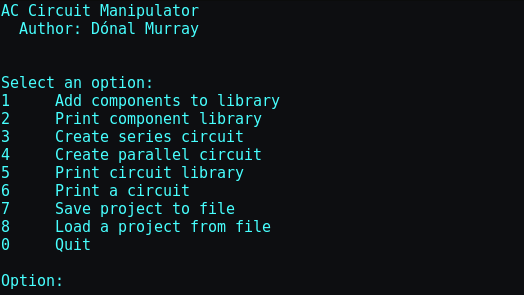
\includegraphics[width=.49\textwidth]{main-menu}
  \end{center}
  \caption{The main menu.}
  \label{fig:menu}
\end{figure}



\begin{figure}[h!]
  \begin{center}
    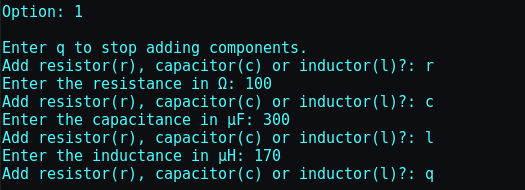
\includegraphics[width=.49\textwidth]{add-comp}
  \end{center}
  \caption{The add component menu.}
  \label{fig:add-comp}
\end{figure}
\begin{figure}[h!]
  \begin{center}
    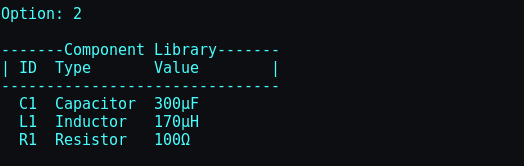
\includegraphics[width=.49\textwidth]{print-comp}
  \end{center}
  \caption{The print component library option.}
  \label{fig:print-comp}
\end{figure}
\begin{figure}
  \begin{center}
    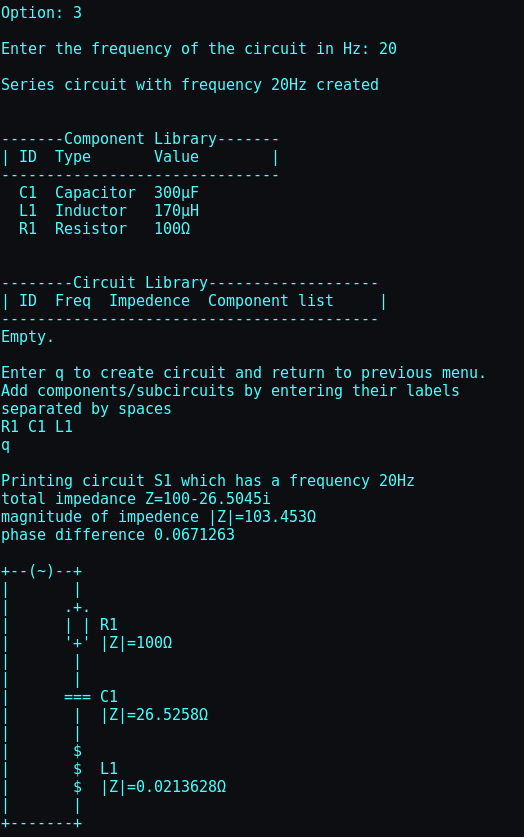
\includegraphics[width=.49\textwidth]{add-series}
  \end{center}
  \caption{The add series circuit menu.}
  \label{fig:add-series}
\end{figure}
\begin{figure}
  \begin{center}
    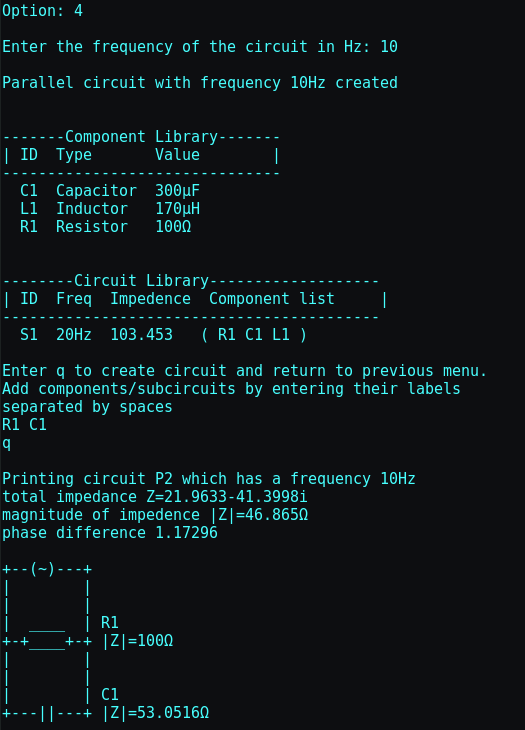
\includegraphics[width=.49\textwidth]{add-parallel}
  \end{center}
  \caption{The add parallel circuit menu.}
  \label{fig:add-parallel}
\end{figure}
\begin{figure}
  \begin{center}
    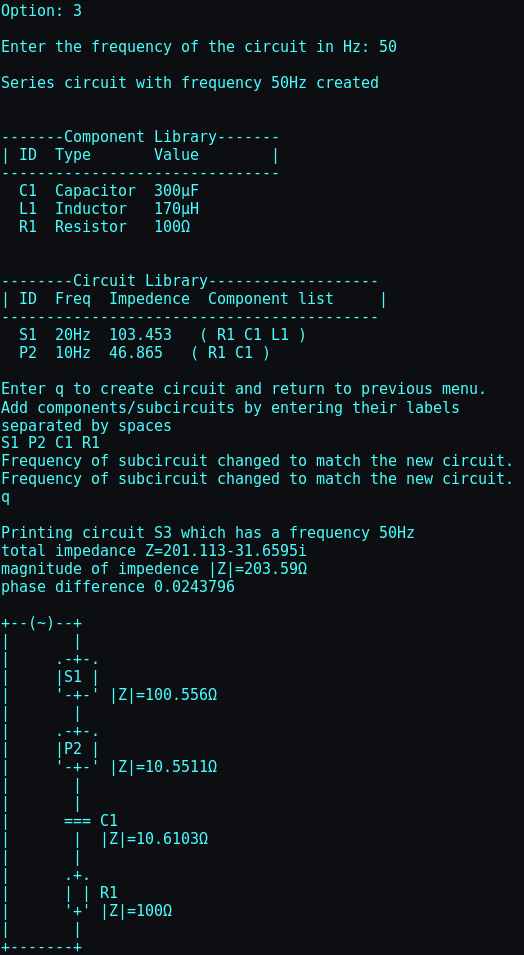
\includegraphics[width=.49\textwidth]{add-nested}
  \end{center}
  \caption{An example of a nested circuit.}
  \label{fig:add-nested}
\end{figure}
\begin{figure}
  \begin{center}
    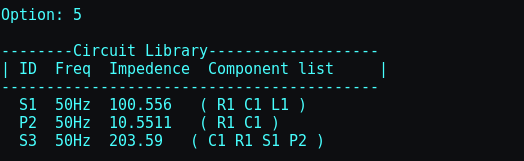
\includegraphics[width=.49\textwidth]{print-circ}
  \end{center}
  \caption{The print circuit library option.}
  \label{fig:print-circ}
\end{figure}
\begin{figure}
  \begin{center}
    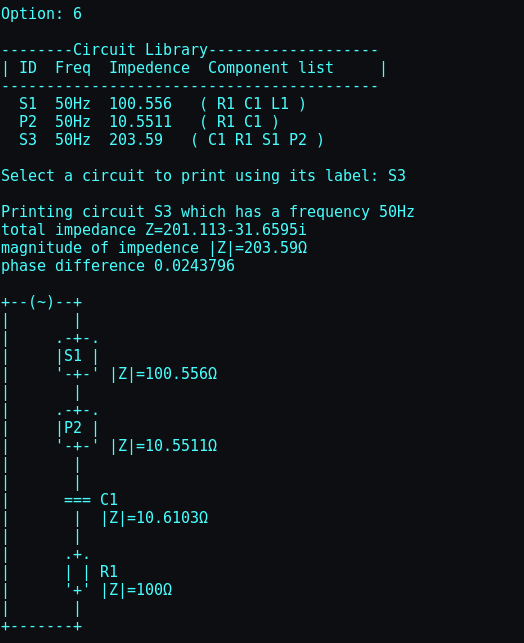
\includegraphics[width=.49\textwidth]{print-circ-diag}
  \end{center}
  \caption{The menu for printing a circuit diagram.}
  \label{fig:print-diag}
\end{figure}
\begin{figure}
  \begin{center}
    
\includegraphics[width=.49\textwidth]{save-proj}
  \end{center}
  \caption{The menu for saving a project to file.}
  \label{fig:save}
\end{figure}
\begin{figure}
  \begin{center}
    
\includegraphics[width=.49\textwidth]{exit}
  \end{center}
  \caption{The exit message.}
  \label{fig:exit}
\end{figure}
\begin{figure}
  \begin{center}
    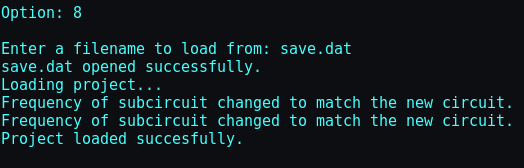
\includegraphics[width=.49\textwidth]{load-proj}
  \end{center}
  \caption{The menu for loading a project from file.}
  \label{fig:load}
\end{figure}
\begin{figure}
  \begin{center}
    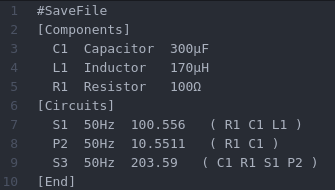
\includegraphics[width=.49\textwidth]{save-format}
  \end{center}
  \caption{An example of a save file.}
  \label{fig:file}
\end{figure}
\clearpage
